\documentclass{grattan_pres}
%\usepackage[utf8]{inputenc}
%\usepackage[T1]{fontenc}

\renewcommand{\mytitle}[1]{\title{#1\vspace{-2ex}}}
\renewcommand{\authors}[1]{\author{#1\vspace{-3ex}}}

\mytitle{Performance}
\authors{Hugh Parsonage}
\date{2018-08-21}

\usepackage{listings}

\providecommand{\Sweavesize}{\smaller}
\providecommand{\Routsize}{\Sweavesize}

\providecommand{\Rcolor}{\color[rgb]{0, 0.5, 0.5}}
\providecommand{\Routcolor}{\color[rgb]{0.461, 0.039, 0.102}}
\providecommand{\Rcommentcolor}{\color[rgb]{0.101, 0.043, 0.432}}

\providecommand{\Rbackground}{\color[gray]{0.91}}
\providecommand{\Routbackground}{\color[gray]{0.935}}
% Can specify \color[gray]{1} for white background or just \color{white}

\lstdefinestyle{Rstyle}{fancyvrb=false,escapechar=`,language=R,%
                        basicstyle={\Rcolor\Sweavesize},% some want \ttfamily too
                        backgroundcolor=\Rbackground,%
                        showstringspaces=false,%
                        keywordstyle=\Rcolor,%
                        commentstyle={\Rcommentcolor\ttfamily\itshape},%
                        literate={<-}{{$\leftarrow$}}2{<<-}{{$\twoheadleftarrow$}}2{~}{{$\sim$}}1{<=}{{$\leq$}}2{>=}{{$\geq$}}2{^}{{$^{\scriptstyle\wedge}$}}1,%
                        alsoother={$},%
                        alsoletter={.<-},%
                        otherkeywords={!,!=,~,$,*,\&,\%/\%,\%*\%,\%\%,<-,<<-,/},%
                        escapeinside={(*}{*)}}%
% Other options of interest:
% frame=single,framerule=0.1pt,framesep=1pt,rulecolor=\color{blue},
% numbers=left,numberstyle=\tiny,stepnumber=1,numbersep=7pt,
% keywordstyle={\bf\Rcolor}
\lstdefinestyle{Routstyle}{fancyvrb=false,literate={~}{{$\sim$}}1{R^2}{{$R^{2}$}}2{^}{{$^{\scriptstyle\wedge}$}}1{R-squared}{{$R^{2}$}}2,%
 frame=single,framerule=0.2pt,framesep=1pt,basicstyle=\Routcolor\Routsize\ttfamily,%
 backgroundcolor=\Routbackground}

 \iffalse $\fi


\usepackage{verbatim}

% \addbibresource{bibliography.bib}

% \makeatletter
% \newbox\@backgroundblock
% \newenvironment{backgroundblock}[2]{%
%   \global\setbox\@backgroundblock=\vbox\bgroup%
%     \unvbox\@backgroundblock%
%     \vbox to0pt\bgroup\vskip#2\hbox to0pt\bgroup\hskip#1\relax%
% }{\egroup\egroup\egroup}
% \addtobeamertemplate{background}{\box\@backgroundblock}{}
% \makeatother

% \newcommand{\lmr}{\fontfamily{lmr}\selectfont}
% \newcommand{\rmLaTeX}{{\lmr\LaTeX{}}}

\hypersetup{colorlinks,linkcolor=black,urlcolor=blue}
\urlstyle{same}

\begin{document}
\section{Performance}
\maketitle

\begin{frame}{Why care about performance}
	\begin{itemize}
		\item Ask more questions 
		\item Ask questions of more data
		\item Provide answers faster
		\item Fewer `interruptions': the difference bewtween a runtime of one second and one minute is \emph{much} more than 59\,seconds.
	\end{itemize}
\end{frame}

\begin{frame}[t]{The Golden Rules of Performance}

\begin{enumerate}\fontsize{11pt}{25}\selectfont
	\item<1-> \textbf{Measure}%\only<2->{\quad }
	\item<3-> \textbf{Don't waste timing saving time}
	% 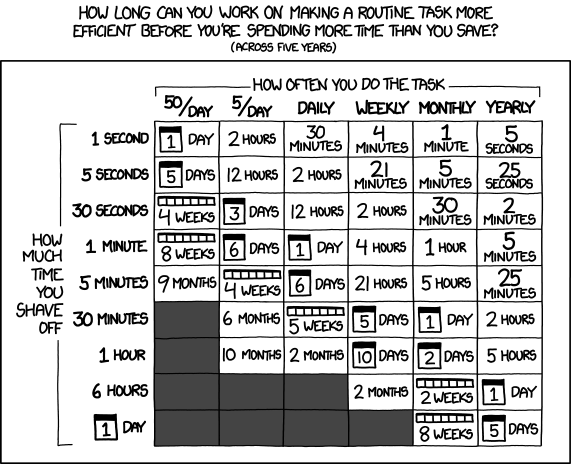
\includegraphics[width=0.5\textwidth]{is_it_worth_the_time.png}
	\item<4-> \textbf{Don't be wrong}
\end{enumerate}

\end{frame}

\begin{frame}[t,fragile]{Measure}
\null\par

	\begin{enumerate}
		\item how long it currently takes
		\item how long it should take
		\item how long your improvement takes
\end{enumerate}

\begin{lstlisting}[style=Rstyle]
x <- rnorm(1e8)
bench::system_time(mean(x))
bench::mark(mean(x), sum(x) / length(x))
library(microbenchmark)
microbenchmark(mean(x), sum(x) / length(x))
\end{lstlisting}

\end{frame}

% \begin{frame}{h}
% 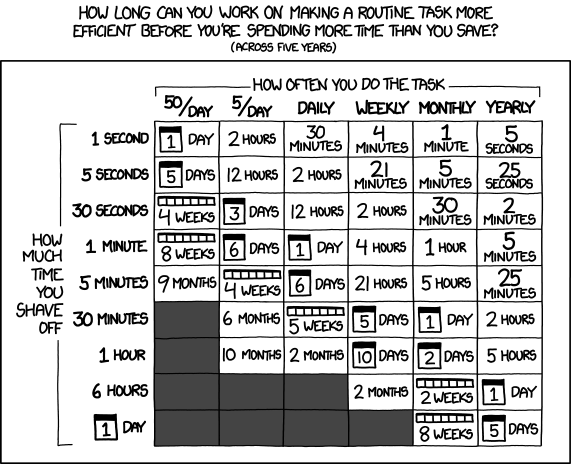
\includegraphics[width=0.5\textwidth]{is_it_worth_the_time.png}

% \end{frame}




\end{document}
